\documentclass[handout]{beamer}

\title{Webpack in Python Projects}
\author{David Fischer}
\date{April 27, 2017}

%% Beamer Themes
\usetheme{Berlin}
\usecolortheme{dove}
\usefonttheme{serif}

%% Packages
% Pygments must be accessible to use minted and --shell-escape
%  must be used with pdflatex
\usepackage{minted}
\usepackage{hyperref}
\usepackage[font=scriptsize,labelformat=empty]{caption}


\setbeamertemplate{footline}{
  \hspace*{.2cm}
  \scriptsize{
    \insertshorttitle
    \hspace*{50pt}
    \hfill
    \insertframenumber/\inserttotalframenumber
    \hspace*{.2cm}
  }
  \vspace{9pt}
}


\begin{document}

\maketitle


% At the highest of high levels, webpack is a JavaScript command line program
\begin{frame}
\frametitle{}
  {\huge What is webpack?}
\end{frame}


% That's not super helpful
\begin{frame}
  It's a ``Module Bundler''
\end{frame}


% So it's some sort of asset pipeline for web assets
% Enough with the buzzwords...
% Webpack takes your source files -- specifically your static files -- and
% processes them so that they are ready for serving in production.
\begin{frame}
  \begin{figure}[p]
    \centering
    \fbox{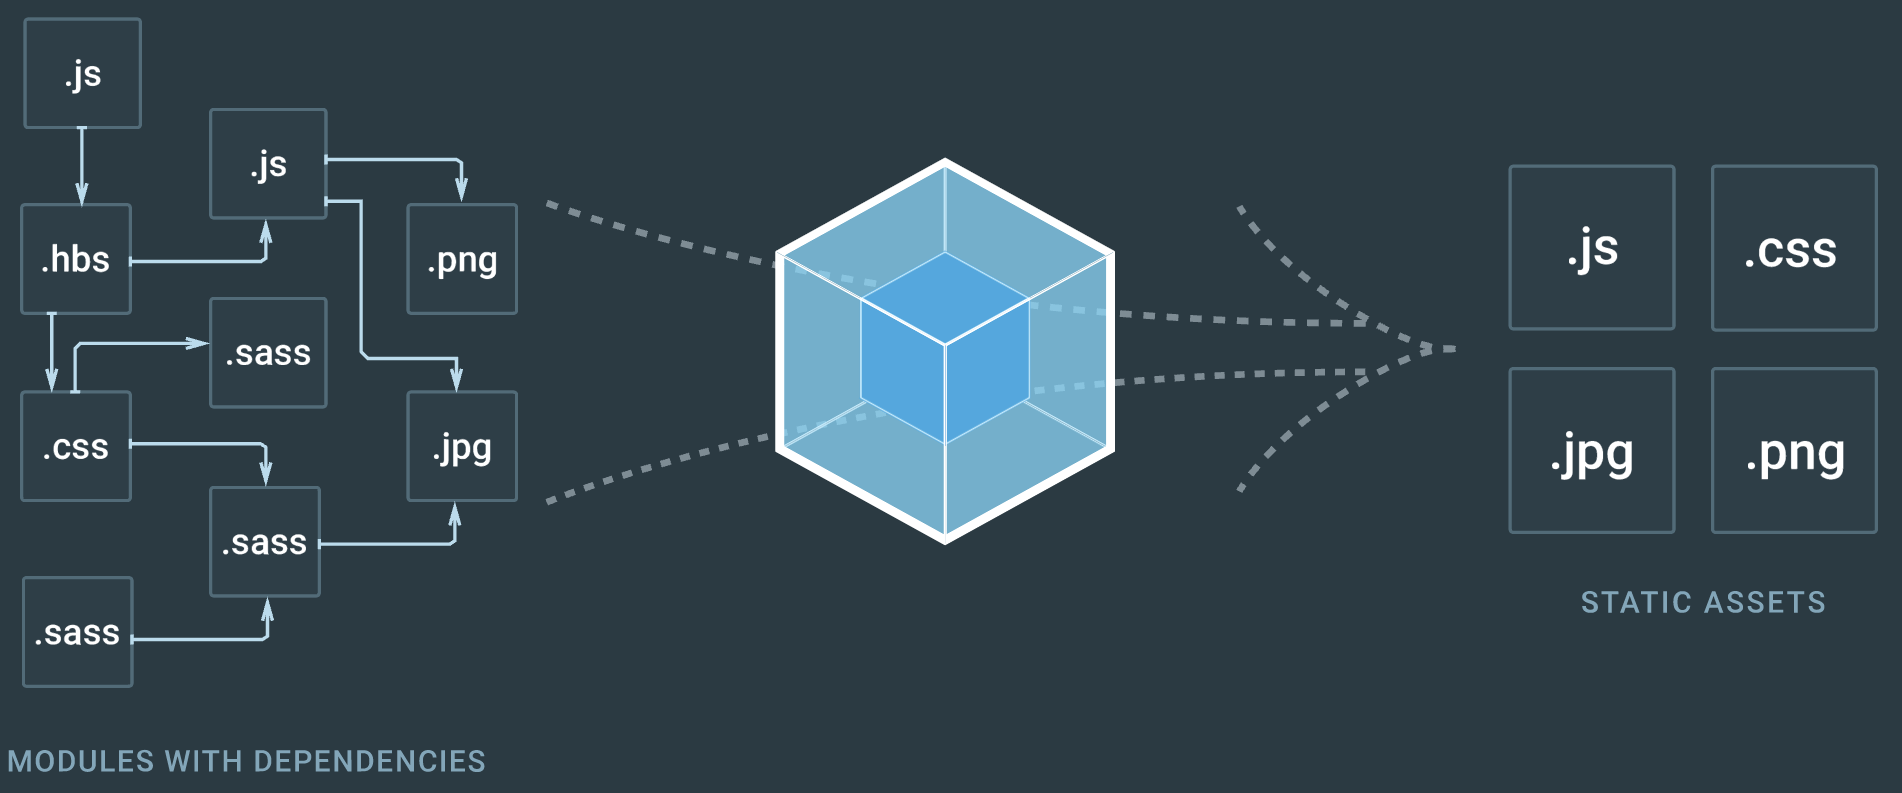
\includegraphics[width=0.8\paperwidth]{includes/webpack.png}}
    \caption{Webpack: the ``bundler''}
  \end{figure}
\end{frame}


% Here's an example in webpack of a simple file processor for image files
% It simply puts all the image files (encountered through CSS, etc.) into
% a single output directory
% This would automatically rewrite any referencing CSS files
% (output not source)to reference the correct path

% Fragile is required for syntax highlighting
\begin{frame}[fragile]
\frametitle{Webpack Configuration}

{\scriptsize
\begin{minted}{javascript}
/// webpack.config.js

module.exports = {
  module: {
    rules: [{
      // When image files are encountered:
      //  - write the images to OUTPUT_DIR/img
      test: /\.(png|gif|jpg|jpeg)$/,
      loader: 'file-loader?name=./img/[name].[ext]'
    }]
  },
  entry: {...},
  output: {...},
};
\end{minted}
}

\end{frame}


% I wanted to highlight some possibilities with a tool like webpack
% **minification** (smaller JS/CSS files) results in faster downloads and faster parsing of your static files
% **file combining** (combining multiple JS/CSS files) results in faster downloads although this is less of an advantage with HTTP2
% **dependency management** - rather than copying bootstrap or jquery into your source tree, there's simply an entry in `package.json`. You use requirements files for python right?
% **caching** - having few static asset bundles with unique hashes allows setting very long expiry headers which results in faster sites
% **standards** - write code using the latest standards while maintaining compatibility with old browsers
\begin{frame}
\frametitle{Please Wait... System Processing...}
  {\scriptsize
    \begin{itemize}
      \item {When webpack encounters Less/SASS/SCSS/CSS files, pre-process them and bundle them into a single output CSS file}
      \item {When webpack encounters image files, use an image minifier (eg. pngquant) to make them smaller, then inline images below a certain file size, and write the remaining images to the output directory rewriting the paths in any referencing files.}
      \item {When webpack encounters JavaScript files, transpile them from the latest JavaScript standards (or TypeScript) to maximize browser compatibility, and then bundle them into a single compressed output JS file.}
      \item {Many more possibilities...}
    \end{itemize}
  }
\end{frame}


\begin{frame}
  Is this a Python talk?
\end{frame}


% I'll show an example of using this with Django
% It's not *that* different with other frameworks
% Largely it is just a matter of serving static files at this point

% Fragile is required for syntax highlighting
\begin{frame}[fragile]
\frametitle{Webpack and Django}

{\scriptsize
\begin{minted}{python}
### settings.py

# STATIC FILES (CSS, JavaScript, Images)
# https://docs.djangoproject.com/en/1.11/howto/static-files/
STATIC_URL = '/static/'
STATIC_ROOT = os.path.join(BASE_DIR, 'static')
STATICFILES_DIRS = (
    # OUTPUT_DIR of webpack
    os.path.join(BASE_DIR, 'assets', 'output'),
)
# http://whitenoise.evans.io/  -  perhaps another talk
STATICFILES_STORAGE = \
    'whitenoise.storage.CompressedManifestStaticFilesStorage'

# An alternative
# STATICFILES_STORAGE = \
    'django.contrib.staticfiles.storage.ManifestStaticFilesStorage'
\end{minted}
}
\end{frame}


% I will put a link to this talk in the comments of the meetup
% Here are links to some other resources

\begin{frame}
\frametitle{Resources}
  \begin{itemize}
    \item {\small Boilerplate to help get started - \href{https://github.com/davidfischer/django-webpack-boilerplate}{github.com/davidfischer/django-webpack-boilerplate}}
    \item {\small A Python helper module for Django - \href{https://github.com/ezhome/django-webpack-loader}{github.com/ezhome/django-webpack-loader}}
    \item {\small Webpack - \href{https://webpack.js.org/}{webpack.js.org}}
    \item {\small Whitenoise (serving static files in Django) - \href{http://whitenoise.evans.io/}{whitenoise.evans.io}}
  \end{itemize}
\end{frame}


\end{document}
